\documentclass{VUMIFPSkursinis}
\usepackage{algorithmicx}
\usepackage{algorithm}
\usepackage{algpseudocode}
\usepackage{amsfonts}
\usepackage{amsmath}
\usepackage{bm}
\usepackage{caption}
\usepackage{color}
\usepackage{float}
\usepackage{graphicx}
\usepackage{listings}
\usepackage{subfig}
\usepackage{wrapfig}
\usepackage{pdflscape} %Keep it to pdflscape or I can't rotate my diagram (K.S.)
\usepackage{longtable}
\usepackage[table]{xcolor}
\usepackage{multirow}
\usepackage[usestackEOL]{stackengine}
\usepackage{longtable}
\usepackage{subfig}
\usepackage{wrapfig}


\usepackage{enumitem}
%PAKEISTA, tarpai tarp sąrašo elementų
\setitemize{noitemsep,topsep=0pt,parsep=0pt,partopsep=0pt}
\setenumerate{noitemsep,topsep=0pt,parsep=0pt,partopsep=0pt}

% Titulinio aprašas
\university{Vilniaus universitetas}
\faculty{Matematikos ir informatikos fakultetas}
\department{Programų sistemų katedra}
\papertype{Programų sistemų inžinerijos laboratorinis darbas Nr. 3}
\title{Kavinės staliuko rezervavimo aplikacija}
\titleineng{Cafe table rezervation app}
\status{2 kurso 5 grupės studentai}
\author{Paulius Grigaliūnas}
\secondauthor{Karolis Staskevičius}
\thirdauthor{Modestas Dulevičius}
\fourthauthor{Albert Jurkoit}
\fifthauthor{Šarūnas Kazimieras Buteikis}
     

% \secondauthor{Vardonis Pavardonis}   % Pridėti antrą autorių
\supervisor{dr. Vytautas Valaitis}
\date{Vilnius – \the\year}

% Nustatymai
% \setmainfont{Palemonas}   % Pakeisti teksto šriftą į Palemonas (turi būti įdiegtas sistemoje)

\begin{document}
% PAKEISTA	
\maketitle
\cleardoublepage\pagenumbering{arabic}
\setcounter{page}{2}


%ANOTACIJA

\sectionnonum{ANOTACIJA}
\noindent


%TURINYS(TOC)
\tableofcontents

%ĮVADAS
\sectionnonum{Įvadas}
\noindent

\section{Verslo proceso aprašas}

\section{Išorinė analizė}

\section{Vidinė proceso analizė}

Šiame skyriuje atliekama vidinė verslo proceso analizė, siekiant nustatyti kavinės rezervavimo programėles stiprybes ir silpnybes, kylančias iš paties verslo proceso (ne jo aplinkos).\\\\

\subsection{Pagrindinės dalykinės srities esybės}
\noindent \textbf{Kavinė} - maitinimo paskirties įstaiga.\\
\textbf{Kavinės} savininkas -asmuo, kuriam priklauso kavinė.\\
\textbf{Klientas} - asmuo, rezervavęs staliuką. \\
\textbf{Maisto tiekėjas} - įmonė, iš kurios kavinė gauna reikalingas prekes ir produktus. \\
\textbf{Rezervacija} - nutarimas, leidžiantis klientui iš anksto turėti konkretų staliuką tam tikru laiku. \\
\textbf{Staliukas} - vieta, prie kurios klientas sėdi restorane.\\
\textbf{Virtuvė} - vieta, kurioje yra ruošiamas užsakymas kavinėje.\\
\textbf{Sąskaita} - kliento apmokėjimas už užsakymą.\\
\textbf{Darbuotojas} - asmuo, kuris dirba kavinėje ir už tai gauna algą.\\

\begin{landscape}
\subsection{Dalykinės srities statinė struktūra}

	\begin {figure}[H]
	\centering
		\caption{Dalykinės srities statinė struktūra}
		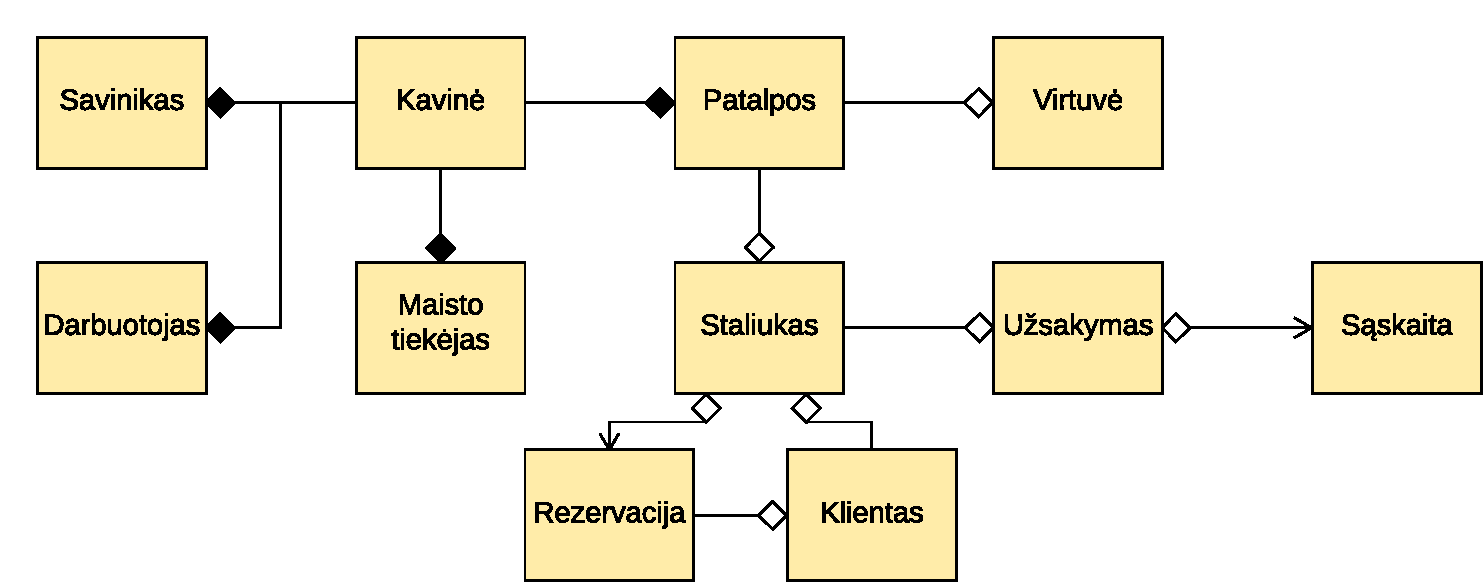
\includegraphics[scale=1]{img/3lab/Diagrama1}
		
		\label{fig:diagrama1}
	\end{figure}
\end{landscape}

Pavaizduota diagrama \ref{fig:diagrama1} pav. pavaizduoja kavinės statinę struktūrą. Kavinė negali egzistuoti be maisto tiekėjų (nebus iš ko ruošti maistą),be darbuotojų (nebus galima efektyviai aptarnauti klientų) ir be kavinės savininko, tad šios esybės sudaro kompoziciją, nes viena negali veikti be kitos.\\
Kavinė gali vykti ir be patalpų, kadangi kavinės staliukai gali stovėti ir 
lauke , todėl šie komponentai sudaro agregaciją.\\
Prie  staliuko  neprivalo  sėdėti  klientas,  nes
staliukas  yra  tik  priemonė  aptarnauti ir jam patogiai jaustis restorane,
klientą.Staliukas taip pat gali nebūti rezervuotas, todėl šios esybės sudaro agregaciją.\\
Patalpose gali būti staliukai ir virtuvė, tačiau tai nėra būtina sąlyga, todėl tai sudaro 
agregaciją.\\
Užsakymas konkretizuoja esybę staliukas.\\
Sąskaita seka po to, kai atliekamas užsakymas.\\

\subsection{Užduočių diagrama}
Klientai  yra  agentai,  kurie  naudodamiesi  kavinės  teikiamomis 
paslaugomis  įgyvendina  užduotis - palydėti  atsisėda  prie  staliuko,  atlieka  užsakymus  ir  juos apmoka. \\
Darbuotojas yra agentas, kuris atlieka tokias užduotis kaip palydėti klientą prie staliuko, 
priimti užsakymą, jį paruošti ir priimti apmokėjimą.\\
Maisto tiekėjas yra agentas, kurio užduotis yra pristatyti reikalingas prekes ir produktus kavinei.\\
Kavinės savininkas valdo kavinės išplanavimą ir staliukų išdėstymą kavinėje. Tik kavinės savininkas gali nuspręsti, kur kavinėje bus išdėstomi staliukai.\\
Agentai ir jų užduotys yra pavaizduoti žemiau esančioje dalykinės srities užduočių diagramoje (žr. \ref{fig:diagrama2} pav).\\


	\begin {figure}[H]
	\centering
		\caption{Dalykinės srities užduočių diagrama}
		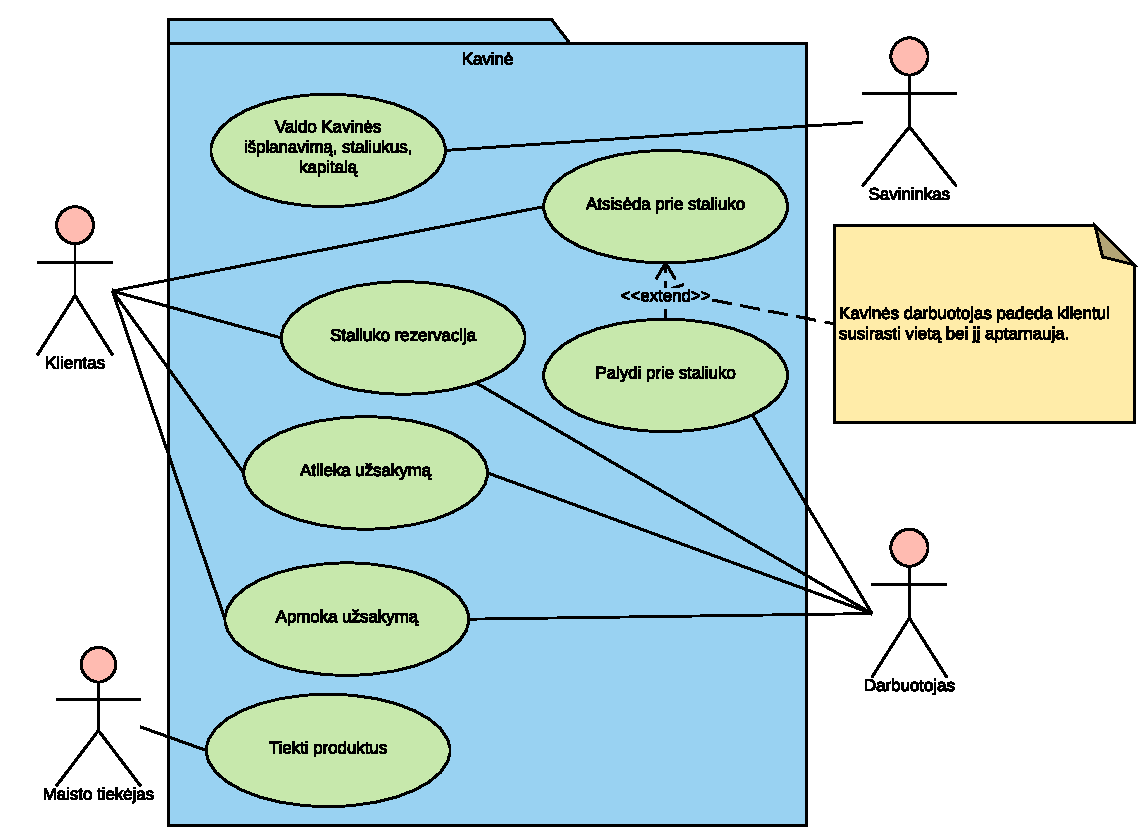
\includegraphics[scale=0.9]{img/3lab/Diagrama2}
		
		\label{fig:diagrama2}
	\end{figure}

\subsection{Užduočių vykdymo scenarijai}
%Insert pauliaus diagram3 here

	\begin {figure}[H]
	\centering
		\caption{Kliento atėjimo į kavinę vykdymo scenarijai}
		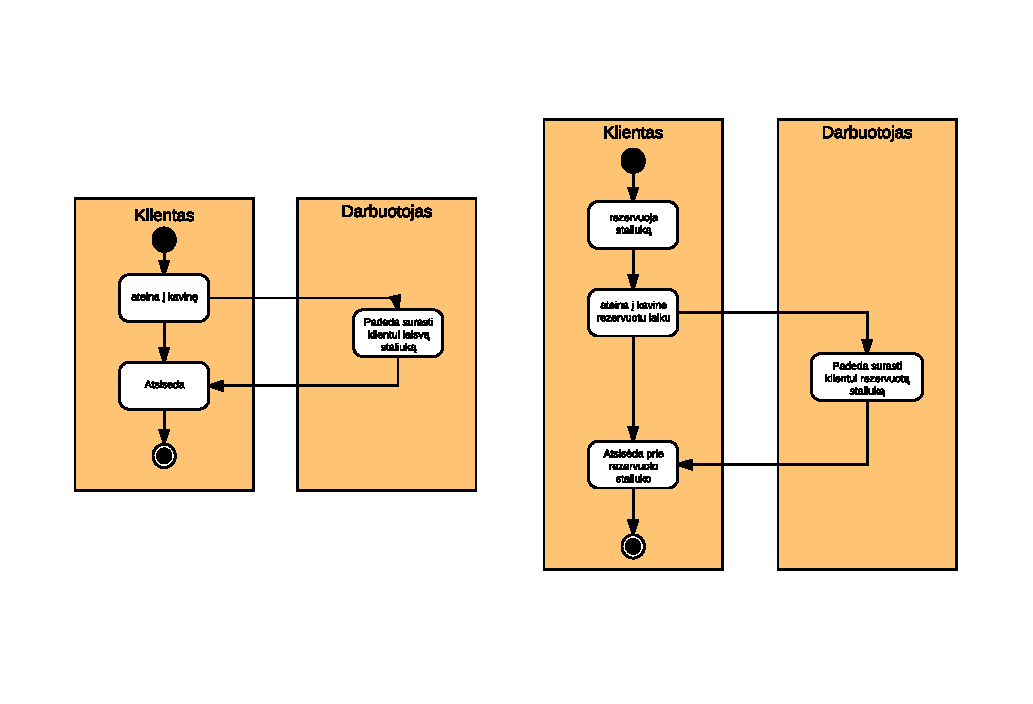
\includegraphics[scale=1]{img/3lab/Diagrama3}
		
		\label{fig:diagrama3}
	\end{figure}

Aukščiau pateiktoje užduočių diagramose (žr. \ref{fig:diagrama3} pav.) pavaizduoti kliento be ir su rezervacija užduočių scenarijai.\\ 
Agentas (klientas) ateina į kavinę ir (turėdamas arba neturėdamas rezervacija) gali paprašyti pagalbos darbuotojo,kad padėtų jam rastų staliuką. Klientas gali ir pats susirasti savo staliuką (klientas, neturėdamas rezervacijos, negali atsisėsti į rezervuotą staliuką). \\
Darbuotojas esant poreikiui iš kliento, padeda jam susirasti norimą staliuką: jeigu klientas turi rezervaciją, tai darbuotojas suranda kliento rezervuotą staliuką, jeigu klientas neturi rezervacijos, tai darbuotojas suranda klientui staliuką, kuris nėra rezervuotas tuo metu.\\

%Insert pauliaus diagram4 here

	\begin {figure}[H]
	\centering
		\caption{kliento aptarnavimo scenarijus}
		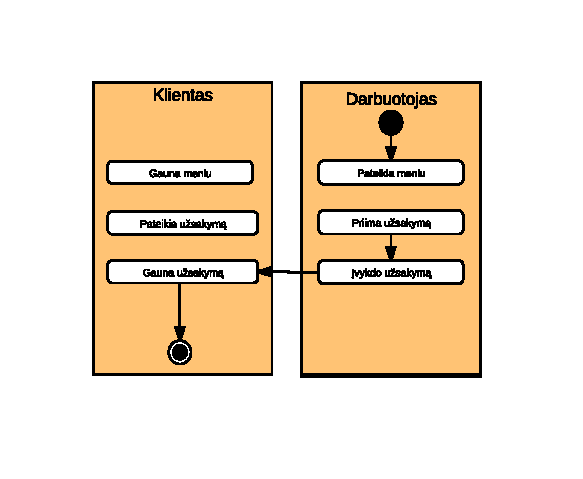
\includegraphics[scale=1]{img/3lab/Diagrama4}
		
		\label{fig:diagrama4}
	\end{figure}
Aukšiau pateiktas kliento aptarnavimo vykdymo scenarijus (žr. \ref{fig:diagrama4} pav.). 
Agentas (darbuotojas) pateikia kitam agentui (klientui) meniu. Gavęs meniu, klientas pateikia 
darbuotojui užsakymą ir šis jį priima. Po to, kai priima užsakymą, darbuotojas jį įvykdo ir tuomet klientas gauna įvykdytą užsakymą. \\

%Insert pauliaus diagram5 here
	\begin {figure}[H]
	\centering
		\caption{kliento atsiskaitymo scenarijus}
		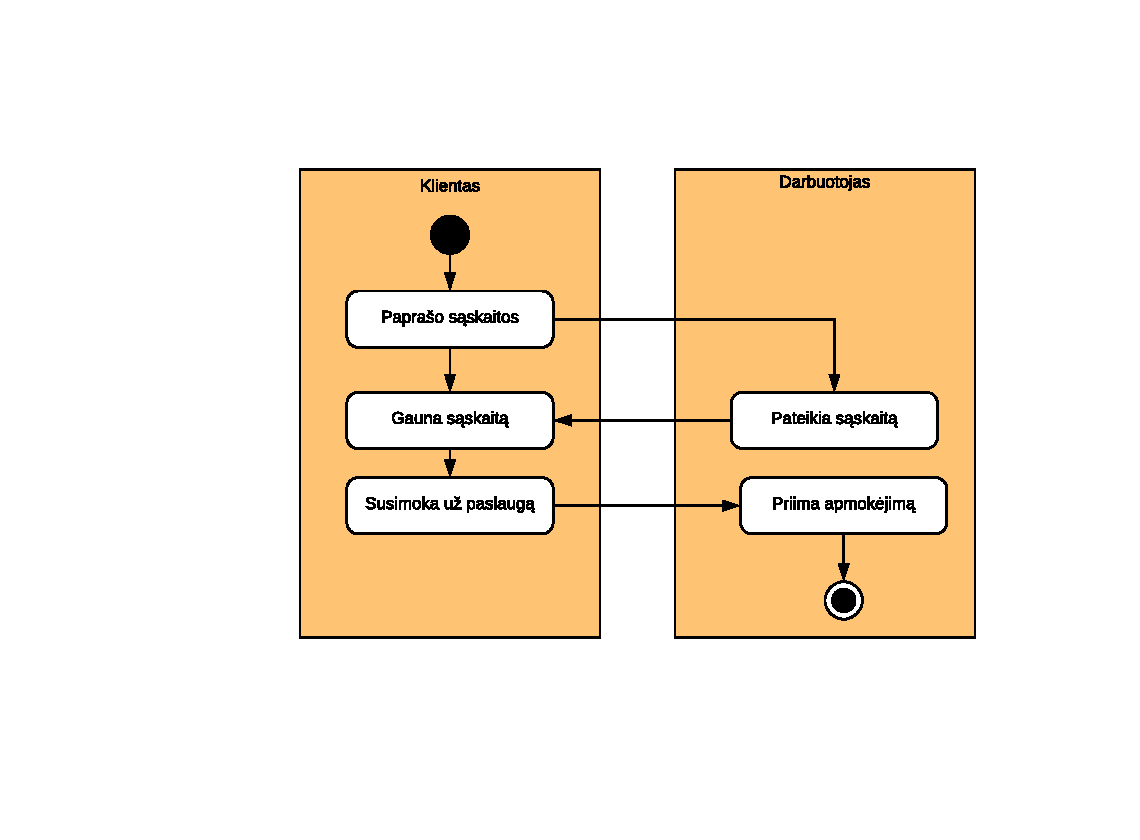
\includegraphics[scale=1]{img/3lab/Diagrama5}
		
		\label{fig:diagrama5}
	\end{figure}
Aukšiau pateiktas kliento atsiskaitymo vykdymo scenarijus (žr. \ref{fig:diagrama5} pav.).
Agentas (klientas) paprašo sąskaitos, tada kitas agentas (darbuotojas) jam ją pateikia. Klientas gauna sąskaitą ir susimoka už jam suteiktas paslaugas. Darbuotojas šį apmokėjimą apdoroja, t.y. jį priima.

%Insert pauliaus diagram 6 here
	\begin {figure}[H]
	\centering
		\caption{Produktų tiekimo į kavinę scenarijus}
		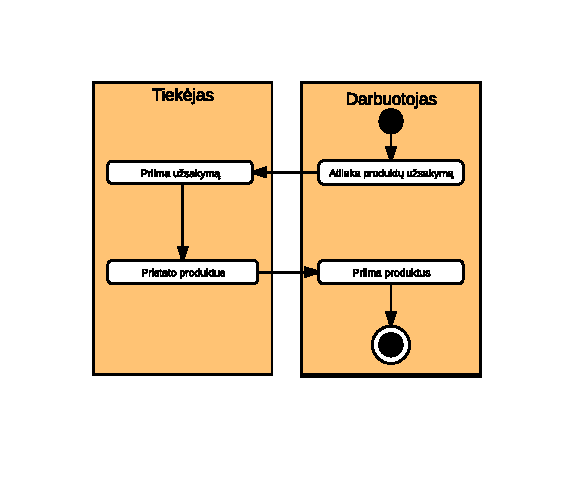
\includegraphics[scale=1]{img/3lab/Diagrama6}
		
		\label{fig:diagrama6}
	\end{figure}
Aukščiau pateiktas reikalingų produktų tiekimo į kavinę scenarijus (žr. \ref{fig:diagrama6} pav.). Agentas (klientas) atlieka kavinei reikiamų produktų užsakymą, tada 
agentas(tiekėjas) jį priima ir pristato produktus. Darbuotojas pristatytus produktus priima. 
\pagebreak
\subsection{Dalykinės srities dinaminė struktūra}

%Insert pauliaus diagram7 here
	\begin {figure}[H]
	\centering
		\caption{Staliuko būsenų diagrama}
		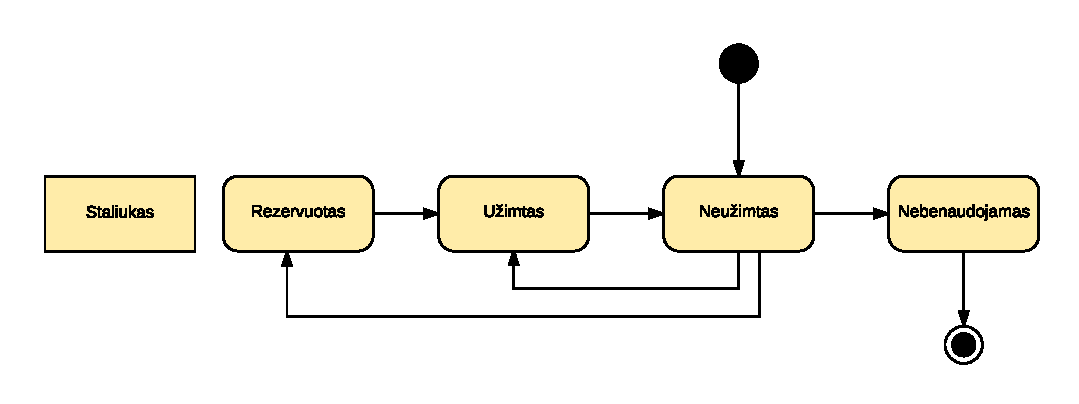
\includegraphics[scale=0.9]{img/3lab/Diagrama7}
		
		\label{fig:diagrama7}
	\end{figure}
		
Pradinė  staliuko  būsena (žr. \ref{fig:diagrama7} pav.)  - neužimtas.  Iš  šios  būsenos  staliukas  gali  tapti  užimtas  arba nebenaudojamas. Iš būsenos užimtas staliukas gali pereiti tik į būseną užimtas. 


%Insert pauliaus diagram8 here

	\begin {figure}[H]
	\centering
		\caption{Užsakymo būsenų diagrama}
		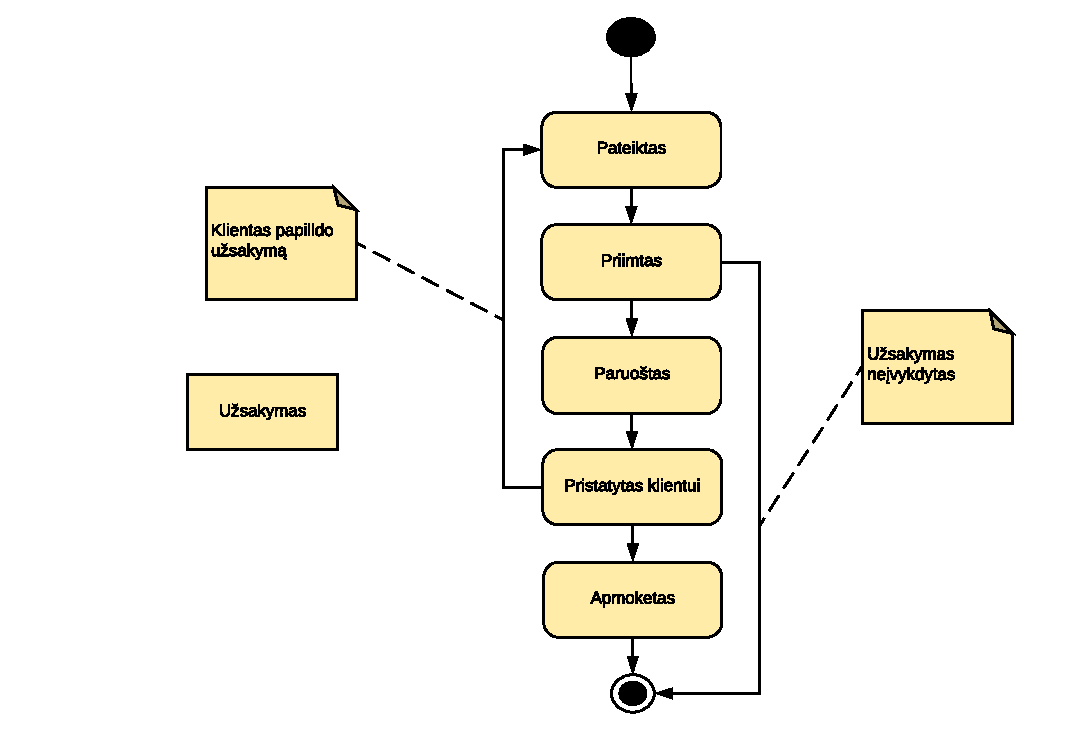
\includegraphics[scale=0.9]{img/3lab/Diagrama8}
		
		\label{fig:diagrama8}
	\end{figure}

Pradinė užsakymo būsena (žr. \ref{fig:diagrama8} pav.) - “pateiktas”, kadangi užsakymas pradeda egzistuoti, kai klientas jį pateikia darbuotojui. Darbuotojui užsirašius ir perdavus užsakymą virtuvei, jis pereina į būseną “priimtas”. Jei užsakymas neįvykdytas, jis nustoja galioti, kitu atveju užsakymas  tampa “paruoštas”. Paruoštas užsakymas yra pristatomas klientui ir keičia būseną į “pristatytas klientui”. Šis turi galimybę arba užsisakyti ką nors papildomai, arba apmokėti sąskaitą. Kai sąskaita apmokama, būsena pasikeičia į „apmokėtas“.\\
\section{Analizės rezultatai}

Šiame skyriuje vidinė ir išorinė verslo proceso analizė apibendrinama pateikiant esmines įžvalgas SSGG (SWOT) lentelės pavidalu. Lentelėje struktūrizuotai pateikiamos verslo stiprybės, silpnybės, jam kylančios grėsmės ir atsiradusios neišnaudotos galimybės (žr. \ref{fig:diagrama9} pav.).

	\begin {figure}[H]
	\centering
		\caption{SWOT lentelė}
		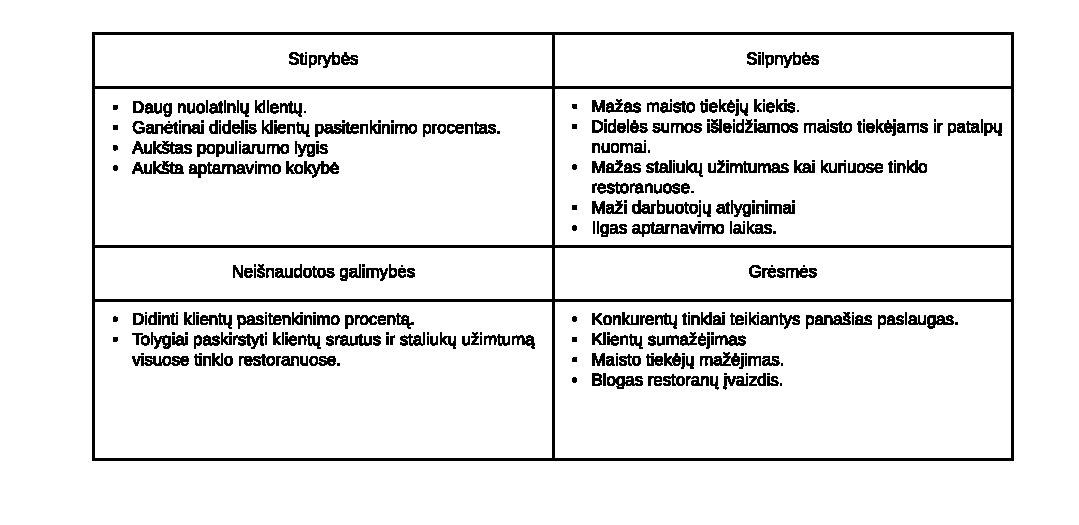
\includegraphics[scale=1]{img/3lab/Diagrama9}
		
		\label{fig:diagrama9}
	\end{figure}

\section{Verslo proceso tobulinimo strategija}
\noindent \textbf{Vizija}.\\
Visi restorano maisto užsakymo ir tiekimo komponentai(užsakymai vietoje, telefonu, internetu, mobilia programėle, maisto tiekimas vietoje bei į namus) turi atnešti pelno restoranui.\\
\textbf{Misija}.\\
Gerinti maisto tiekimo sąlygas klientams, naudojantis šiuolaikinėmis technologijomis, tobulinti mažiau pelningus komponentus.\\
\textbf{Tikslai/Siekiai}.\\
Didinti restorano staliukų užimtumą, lanksčiai paskirstant klientų srautus:
	\begin{itemize}
	\item Gerinti maisto kokybę ieškaint naujų tiekėjų;
	\item Sumažinti klientų aptarnavimo trukmę;
	\item Pagerinti klientų aptarnavimo kokybę;
	\item Didinti algas restorano darbuotojams;
	\item Didinti klientų užimtumą laukimo metu (plėsti pramogų skaičių, tokių kaip mokami stalo žaidimai ir kt.);
	\end{itemize}
Plėsti užsakymo „iš namų“ sistemą, kuriant internetinę svetainę ar mobilią programėlę, kurios leistų:
	\begin{itemize}
	\item Žemėlapyje parodytų arčiausiai esančius restoranus ir jų laisvų staliukų skaičių;
	\item Matyti restorano staliukų išplanavimą bei kurie staliukai restorane nėra užimti,
	\item Rezervuoti staliuką restorane norimu laiku tam tikroje vietoje;
	\end{itemize}

\section{Sistemos naudojimo scenarijus}

Šiame skyriuje yra aprašyti sistemos teikiama nauda bei žemiau pateiktas sistemos naudojimo scenarijus (žr \ref{fig:maincase} pav.).

% čia reikia imest diagrama MainCase.jpg
\subsection{Naudojimo scenarijus}
	\begin {figure}[H]
	\centering	
		\caption{pagrindinis sistemos naudojimo scenarijus}
		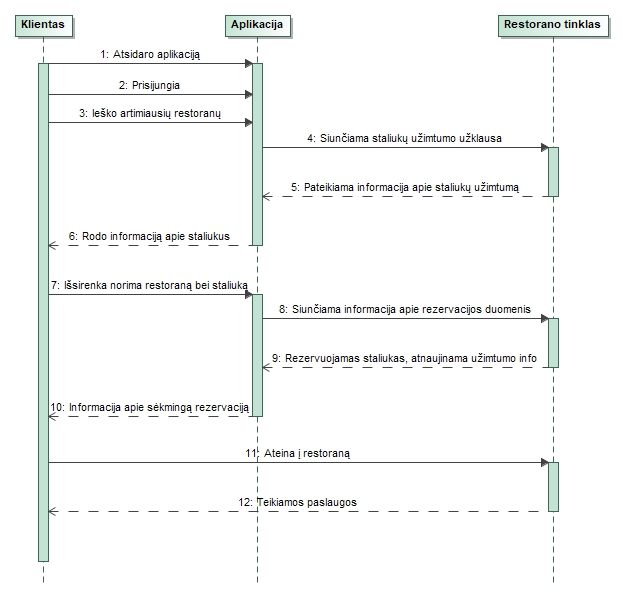
\includegraphics[scale=0.7]{img/3lab/MainCase.jpg}
		
		\label{fig:maincase}
	\end{figure}
Vartotojas atsidaro mobiliąją aplikaciją, įrašytą išmaniajame telefone arba planšetėje. Ivedęs prisijungimo duomenis jis patenka į pagrindinį langą, kuriame gali ieškoti artimiausiai esančių restoranų pagal vartotojo esamą lokaciją. Aplikacija siunčia užklausą į restoranų tinklą apie restoranų užimtumą. Vartotojui pateikiamas sąrašas restoranų su informacija apie esamus laisvus ir užimtus staliukus. Vartotojas išsirenką jam tinkantį restoraną ir pasirenką staliuką, kurį norėtų rezervuoti. Duomenys apie rezervavimą yra siunčiami restoranų tinklui, kuriame vyksta staliuko rezervavimas ir atnaujinta informacija siunčiama aplikacijai. Vartotojui yra pateikiama informaciją apie sėkmingai rezervuotą staliuką. Jam lieka tik ateiti į restoraną ir jam yra teikiamos paslaugos, kurios buvo numatytos užsakymo informacijoje.

\subsection{Sistemos teikiama nauda}

Žemiau pateiktoje diagramoje yra pavaizduoti sistemos naudojimo privalumai (žr \ref{fig:systemusingbenefits} pav.).
% čia reikia įmest diagramą SystemUsingBenefits.jpg

	\begin {figure}[H]
	\centering	
		\caption{Systemos naudojimo scenarijus}
		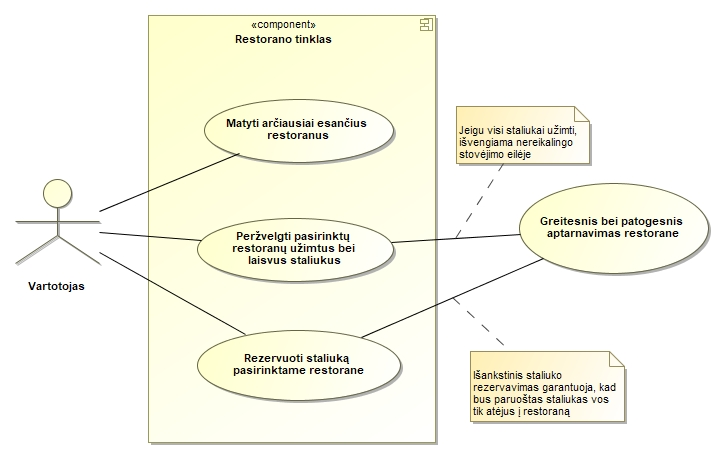
\includegraphics[scale=0.7]{img/3lab/SystemUsingBenefits.jpg}
		
		\label{fig:systemusingbenefits}
	\end{figure}

Vartotojas gali matyti arčiausiai jo esančius restoranus. Taip pat jis turi galimybę matyti užimtus bei laisvus restoranų staliukus, kas leidžia išvengti bereikalingo stovėjimo eilėje, jeigu visi staliukai užimti. Be šių privalumų, vartotojas gali iš anksto užsirezervuoti staliuką norimame restorane ir užsitikrinti, kad vos tik atvykus į restoraną jam bus paruoštas rezervuotas staliukas bei nereikės laukti.

\subsection{Esama būklė}

Mobiliajai aplikacijai „Covfefe“ realizuoti gali reikėti:
\begin{itemize}
\item Interneto ryšio.
\item Serverio, kuriame būtų saugomi duomenys apie klientus bei staliukų rezervaciją.
\item Restoranų tinkle įdiegtos programinės įrangos, galinčios siųsti duomenis apie restorano staliukų pozicijas bei jų užimtumą.
\item Žmonių, galinčių įdiegti ir tvarkyti sistemą.
\item Mobiliosios aplikacijos.
\end{itemize}


\subsection{Priemonės scenarijui įgyvendinti}

Priemonės, reikalingos sistemos scenarijui įgyvendinti:
\begin{itemize}
\item Interneto priegos.
\item Naujos darbo vietos technikai įtaisyti ir prižiūrėti.
\item Darbuotojų apmokymo.
\item Algoritmo, randančio arčiausiai esančius restoranus su jų laisvų staliukų skaičiais.
\item Duomenų bazės, kurioje būtų saugomos lentelės su klientų informacija bei staliukų rezervacijomis.

\end{itemize}

 \section{Įgyvendinamumo ir naudos analizė}
Šiame skyriuje bus analizuojamas sistemos įgyvendinamumas ir jos nauda.
\subsection{Operacinis įgyvendinamumas}
Inovaciniai slenksčiai:\\
Darbuotojai su žemu kompiuteriniu raštingumu gali nemokėti naudotis nauja programine įranga arba
nenorėti prisitaikyti prie pokyčių.\\
Klientai, nepratę prie naujos aplikacijos, gali nežinoti, kaip ji tiksliai veikia ir ja nesinaudoti.\\
\\
Šių inovacinių slenksčių panaikinimo būdai:\\
Darbuotojams vesti mokymus, paaiškinti apie sistemos teikiama naudą darbuotojams, geriausiai ir
greičiausiai prisitaikiusiems prie naujos aplikacijos mokėti priedus.\\
Naujai aplikacijai sukurti ir taikyti reklamos strategiją\\
Klientams sukūrti demonstracinį video įrašą, kuris supažindins su sistemos pagrindiniais panaudojimo scenarijais.

\subsection{Techninis įgyvendinamumas}
Kompiuteris su Windows OS ir bent:\newline
{\begin{itemize}
\item 2048MB RAM
\item 20GB HDD
\item 1700MHz procesoriumi
\end{itemize}

\subsection{Ekonominis įgyvendinamumas}
Reikalinga techninė įranga (serveriui):
{\begin{itemize}
\item Kompiuteris - 1000 eur
\item Nepertraukiamo maitinimo šaltinis - 180 eur
\item Tinklo įranga - 30 eur
\item Iš viso: 1210 eur
\end{itemize}
\hfill\break


Reikalinga techninė įranga (vienam restoranui):

{\begin{itemize}
\item Kompiuteris - 500 eur 
\item Nepertraukiamo maitinimo šaltinis - 180 eur
\item Iš viso: 680 eur
\end{itemize}
\break

Programinė įranga:
{\begin{itemize}
\item Operacinė sistema Windows 10 Pro - 200 eur 
\item Sistema „Covfefe“ - 10 000 eur
\item Iš viso: 10 200 eur
\end{itemize}
\hfill\break

Bendra įrangos kaina - 12 090 eur

Metinės eksplotavimo išlaidos:
{\begin{itemize}
\item Atlyginimas sistemos administratoriui - 7 200 eur
\item Interneto paslaugos - 1000 eur
\item Programinės ir techninės įrangos aptarnavimas ir atnaujinimas - 5000 eur
\item Iš viso: 13200 eur per metus
\end{itemize}
\hfill\break

Numanoma verslui atnešama nauda:\\
Registruotose restoranuose (orientuojamasi į 60 registruotų restoranų tinklą) apsilanko 250000 žmonių per mėnesį. Per metus registruotu restoranų tinklas gauna 600000
eur pelno.\\
Įdiegus sistemą “Covfefe” tikimasi padidinti staliukų užimtumą 15\% ir taip padidinti
pelną 90000 eur per metus.
\hfill\break

Sistema atsipirktų po 8 menėsių. 

\subsection{Juridinis įgyvendinamumas}
Sukuriant sistemą nebus pažeista Lietuvos respublikos konstitucija, Asmens duomenų
apsaugos įstatymas, Statistikos įstatymas ar kitų Lietuvos Respublikos teisės aktų numatyti
draudimai.\\
 Darbuotojai turi teisę į tinkamas, saugias ir sveikas darbo sąlygas. Darbuotojams
mokamas menėsinis atlyginimas, darbo valandos neviršija 8 valandų per parą. Kiekvienas
darbuotojas turi teisę į poilsį ir laisvalaikį, taip pat kasmetines mokamas atostogas.\\ 
Duomenys tvarkomi tiksliai, sąžiningai ir konfidencialiai.
\break

\section{Literatūros sąrašas}
\begin{itemize}
\item MOBILIŲJŲ APLIKACIJŲ KŪRIMO KAINA http://descode.lt/mobiliuju-aplikaciju-kurimo-kaina/
\end{itemize}


\end{document}
